%!TEX root = ../thesis.tex

\section{提案手法の概要}

  本研究は,ルールベース制御器に引き紐ではなく,2DLiDARの反射強度を利用する.このときのロボットの行動を\figref{Fig:RobotGuidance_velocity}に示す.並進速度は,学習時と学習後で共に0.2 \,[m/s]で一定で,ロボットのヨ―方向の角速度$\omega$のみ変化する.ルールベース制御器は,追従対象者に再帰反射テープを装着し,2DLiDARでそれを検出することで,人に追従する手法である.

  \begin{figure}[h]
    \centering
    \begin{minipage}[c]{65mm} 
        \centering
        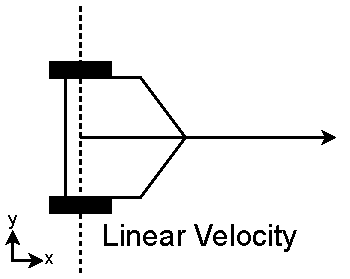
\includegraphics[height=40mm]{images/pdf/RobotGuidance_linear_velocity}
        \subcaption{Forward is fixed}
    \end{minipage}
    \begin{minipage}[c]{65mm} 
        \centering
        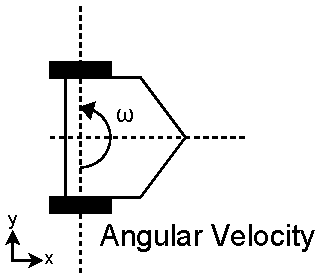
\includegraphics[height=40mm]{images/pdf/RobotGuidance_angular_velocity}
        \subcaption{Angular velocity changes depending on input}
    \end{minipage}
    \caption{Output robot actions}
    \label{Fig:RobotGuidance_velocity}
  \end{figure}

\newpage

  深層学習器は,ルールベース制御器の出力(ロボットのヨ―方向の角速度$\omega$)とRGB画像をend-to-end学習することで,\figref{Fig:RobotGuidance_simple_system}に示すように,入力をRGB画像,出力をロボットのヨ―方向の角速度$\omega$として人を追従する.

  \begin{figure}[h]
    \centering
    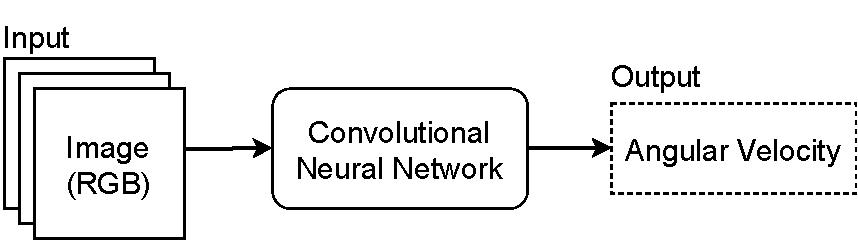
\includegraphics[keepaspectratio, scale=0.50] {images/pdf/RobotGuidance_simple_system}
    \captionsetup{justification=raggedright} % キャプションを左寄せに
    \caption{The trained network is used to generate the robot's yaw angular velocity from the RGB images}
    \label{Fig:RobotGuidance_simple_system}
  \end{figure}

  \figref{Fig:RobotGuidance_all_system}に示すように,ルールベース制御器を用いてロボットを制御するフェーズを学習フェーズ,深層学習器の出力をロボットの行動にするフェーズを追従フェーズと呼ぶこととする.以下に,学習フェーズと追従フェーズの主な役割を示す.

  \subsubsection*{<学習フェーズ>}
  2DLiDARの反射強度を利用したルールベース制御器に従い,ロボットを制御する.制御器の出力と画像を教師信号として深層学習器に与え,オンラインでend-to-end学習する.
  
  \subsubsection*{<追従フェーズ>}
  2DLiDARは使用せず,画像を入力とした深層学習器の出力をロボットの行動にする.つまり,画像に基づいてロボットが人を追従する.

  \begin{figure}[h]
    \centering
    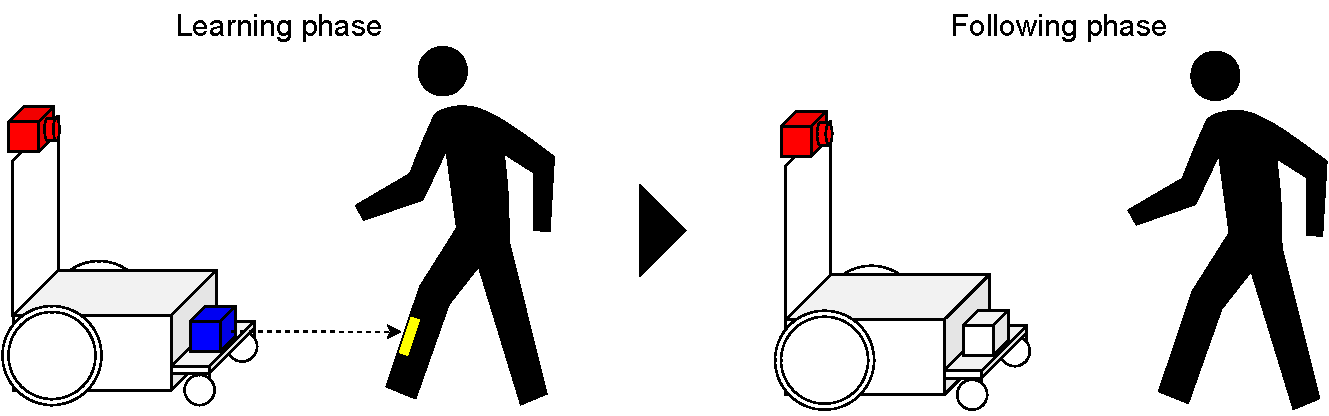
\includegraphics[keepaspectratio, scale=0.35] {images/pdf/RobotGuidance_all_system}
    \captionsetup{justification=raggedright} % キャプションを左寄せに
    \caption{Sequence of proposed method}
    \label{Fig:RobotGuidance_all_system}
  \end{figure}

\newpage
